%% symbol library for TikZ track schematics
%
% Copyright (c) 2018 - 2022 Martin Scheidt (ISC license)

% Permission to use, copy, modify, and/or distribute this file for any purpose with or without fee is hereby granted, provided that the above copyright notice and this permission notice appear in all copies.

\documentclass{scrartcl}

\usepackage{tikz-trackschematic-documentation}

%%%%%% AUTHORS list %%%%%%%%%%

%\newcommand{\initials}{fullname}
\newcommand{\MS}{Martin Scheidt}
\newcommand{\GW}{Gregor Wehrle}
\newcommand{\authorlist}{by the project contributors}

%%%%%%%%%%%%%%%%%%%%%%%%%%%%%%

% -------[ PDF Informations ]---------
\hypersetup{%
  pdftitle={tikz-trackschematic},
  pdfsubject={A tikz toolbox for track schematics},
  pdfauthor={\authorlist},
  pdfkeywords={latex, tikz, library, railway, track layout, schematic}
}

\begin{document}

\title{\color{gray}\Huge\sffamily \{\textcolor{black}{Ti\textcolor{orange}{\emph{k}}Z}-\textcolor{blue}{trackschematic}\}}
\subtitle{A Ti\emph{k}Z library for track schematics}
\author{\authorlist}
\date{Version \vhCurrentVersion~ from \vhCurrentDate}

\maketitle

\begin{multicols}{2}
  \tableofcontents
\end{multicols}
\cleardoublepage

\section{Introduction}\label{sec:intro}

  \subsection{About tikz-trackschematic}

    The Ti\emph{k}Z-\emph{trackschematic} library is a toolbox of symbols geared primarily towards creating track schematic for either research or educational purposes.
    It provides a Ti\emph{k}Z frontend to some of the symbols which maybe needed to describe situations and layouts in railway operation.
    The library is divided into the following sublibraries:
    \begin{itemize}
      \item \texttt{topology},
      \item \texttt{trafficcontrol},
      \item \texttt{vehicles},
      \item \texttt{constructions},
      \item \texttt{symbology},
      \item \texttt{electrics}, and
      \item \texttt{measures}.
    \end{itemize}

  \subsection{Acknowledgement}

    This project has received funding from the European Union’s Horizon 2020 research and innovation programme under grant agreement No. 826347.
    If you want to cite this project please use the follwoing informations:\\
    Scheidt, M. (2021). TikZ-trackschematics (Version \vhCurrentVersion) DOI: 10.5281/zenodo.5539845

  \subsection{Requirements}\label{sec:require}

    The library uses Ti\emph{k}Z and it is based the following packages:
    \begin{itemize}
      \item \texttt{tikz},
      \item \texttt{xcolor}, and
      \item \texttt{etoolbox}.
    \end{itemize}

    Further more it uses the following Ti\emph{k}Z libraries:
    \begin{itemize}
      \item \texttt{calc},
      \item \texttt{intersections},
      \item \texttt{patterns}, and
      \item \texttt{arrows.meta}.
    \end{itemize}


  \subsection{License}

    Copyright (c) 2018 - 2022, \MS.
    Permission to use, copy, modify, and/or distribute this file for any purpose with or without fee is hereby granted, provided that the above copyright notice and this permission notice appear in all copies (\href{https://www.tldrlegal.com/l/isc}{ISC license}).

  \subsection{Alternatives}

    Apart from this library, there is also the \href{https://tu-dresden.de/bu/verkehr/ibv/vst/die-professur/mitarb/ulrich-maschek/signalschablone}{Signalschablone} with german (Deutsche Bahn) symbols for MS Visio.


% \newpage
\section{Usage}\label{sec:use}
  \subsection{A complete minimal example}

    The command \texttt{\textbackslash usepackage\{tikz-trackschematic\}} will load the library; place it somewhere in your preamble.
    Here is a complete working minimal example which will produce a single PDF file with the figure on the right:\\
    \begin{minipage}[c]{0.51\textwidth}
      \centering
      \lstinputlisting{examples/minimal_working_example.tex}
    \end{minipage}
    \hfil
    \begin{minipage}[c]{0.45\textwidth}
      \centering
      \begin{tikzpicture}
        \path (-0.2,-1.45) rectangle (6.2,1.45);
        \coordinate (A) at (0,0);
        \coordinate (T) at (5,0);
        \coordinate (B) at (6,0);
        \maintrack  (A) -- (B);
        \train[forward] at (T) label ();
      \end{tikzpicture}
    \end{minipage}

  \subsection{Placement}\label{sec:placement}

    To place symbols in a track schematic, they need to placed and oriented correctly.
    The placement ist done through the given Ti\emph{k}Z coordinate.
    There are a few assumaptions made about the placement:
    \begin{enumerate}
      \item Parallel tracks are drawn at a distance of 1 cm (which is the base unit of Ti\emph{k}Z).
      \item Tracks are only drawn at an angle of $n \cdot 45^{\circ}$.
    \end{enumerate}

  \subsection{Orientation system}\label{sec:orientationsystem}

    The orientation is controlled via given Ti\emph{k}Z options or pgfkey.
    The orientation options/pgfkeys inhibit their meaning from reading left to right as \texttt{forward} and relate \texttt{left}/\texttt{right} to that movement.
    \begin{center}
      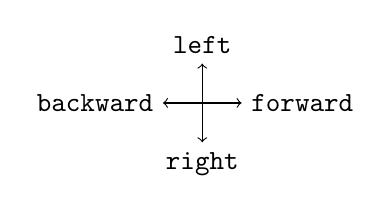
\begin{tikzpicture}[font=\ttfamily]
        \draw[<->] (-0.5,0) node[left]  {backward} -- ++(1,0) node[right] {forward};
        \draw[<->] (0,-0.5) node[below] {right}    -- ++(0,1) node[above] {left};
      \end{tikzpicture}
    \end{center}

    The main option/pgfkey is the \texttt{face} option to control in which direction an object will face.
    The key can take one of the following two values:
    \begin{itemize*}[label={}]
      \item \texttt{forward}, and
      \item \texttt{backward}.
    \end{itemize*}
    \begin{minipage}[c]{0.68\textwidth}
    \begin{lstlisting}[gobble=6]

      \train[face=forward] at (coordinate) label ();

    \end{lstlisting}
    \end{minipage}
    \hfil
    \begin{minipage}[c]{0.30\textwidth}
      \tikz{\train[face=forward] at (5,0) label ();}
    \end{minipage}
    \begin{minipage}[c]{0.68\textwidth}
    \begin{lstlisting}[gobble=6]

      \train[face=backward] at (coordinate) label ();

    \end{lstlisting}
    \end{minipage}
    \hfil
    \begin{minipage}[c]{0.30\textwidth}
      \tikz{\train[face=backward] at (1,0) label ();}
    \end{minipage}
    As a shortcut you may also just give the option \texttt{forward} or \texttt{backward} without the \texttt{face=} in front of it.

    If you have objects which branch either to the left or the right you have to give the \texttt{branch} option which takes one of the following two values:
    \begin{itemize*}[label={}]
      \item \texttt{left}, and
      \item \texttt{right}.
    \end{itemize*}\\
    \begin{minipage}[c]{0.68\textwidth}
    \begin{lstlisting}[gobble=6]

      \turnout[forward ,branch=left ] at (coordinate) label ();

    \end{lstlisting}
    \end{minipage}
    \hfil
    \begin{minipage}[c]{0.30\textwidth}
      \tikz{\maintrack (0,0)--(4,0);\maintrack (2,0)--++(0.5,0.5);\turnout[forward,branch=left] at (2,0) label ();}
    \end{minipage}
    \begin{minipage}[c]{0.68\textwidth}
    \begin{lstlisting}[gobble=6]

      \turnout[forward,branch=right] at (coordinate) label ();

    \end{lstlisting}
    \end{minipage}
    \hfil
    \begin{minipage}[c]{0.30\textwidth}
      \tikz{\maintrack (0,0)--(4,0);\maintrack (2,0)--++(0.5,-0.5);\turnout[forward,branch=right] at (2,0) label ();}
    \end{minipage}
    \begin{minipage}[c]{0.68\textwidth}
    \begin{lstlisting}[gobble=6]

      \turnout[backward,branch=left] at (coordinate) label ();

    \end{lstlisting}
    \end{minipage}
    \hfil
    \begin{minipage}[c]{0.30\textwidth}
      \tikz{\maintrack (0,0)--(4,0);\maintrack (2,0)--++(-0.5,0.5);\turnout[backward,branch=left] at (2,0) label ();}
    \end{minipage}
    \begin{minipage}[c]{0.68\textwidth}
    \begin{lstlisting}[gobble=6]

      \turnout[backward,branch=right] at (coordinate) label ();

    \end{lstlisting}
    \end{minipage}
    \hfil
    \begin{minipage}[c]{0.30\textwidth}
      \tikz{\maintrack (0,0)--(4,0);\maintrack (2,0)--++(-0.5,-0.5);\turnout[backward,branch=right] at (2,0) label ();}
    \end{minipage}
    There is no shortcut and the key \texttt{branch=} must be given contrary to the key \texttt{face=}.

  \subsection{Left- and right-hand traffic}\label{sec:traffic}

    The traffic practice to divide bidirectional traffic has impact mostly on traffic control.
    The default traffic practice for this library ist right-hand traffic.
    You can change it either globally or locally with the key \texttt{traffic practice=left}.
    There is also the alias \texttt{position} for single local entries.
    
    \begin{minipage}[c]{0.65\textwidth}
      \begin{lstlisting}[gobble=8]
        \documentclass{standalone}

        % load the library
        \usepackage{tikz-trackschematic}

        \begin{document}
          \begin{tikzpicture}
            % set the traffic practice
            \tikzset{traffic practice=left}

            \maintrack  (0,1) -- (5,1);
            \maintrack  (0,0) -- (5,0);
            \routesignal[forward]                at (2,1) label (left);
            \routesignal[forward,position=right] at (2,0) label (right);
          \end{tikzpicture}
        \end{document}
      \end{lstlisting}
    \end{minipage}
    \hfil
    \begin{minipage}[c]{0.34\textwidth}
      \begin{tikzpicture}
        \tikzset{traffic practice=left}
        \path (-0.2,-1.6) rectangle (5.2,2.6);
        \coordinate (A1) at (0,1);
        \coordinate (S1) at (2,1);
        \coordinate (B1) at (5,1);
        \maintrack  (A1) -- ( B1);
        \coordinate (A2) at (0,0);
        \coordinate (S2) at (2,0);
        \coordinate (B2) at (5,0);
        \maintrack  (A2) -- ( B2);
        \routesignal[forward] at (S1) label (left);
        \routesignal[forward,position=right] at (S2) label (right);
      \end{tikzpicture}
    \end{minipage}

  \subsection{Colors: background and foreground}\label{sec:colors}

    The two main colors \texttt{white} and \texttt{black} are set for the \texttt{background} and \texttt{foreground} keys by default.
    If you want to change them, provide a new value for the keys.
    For example like this:\\
    \begin{minipage}[c]{0.65\textwidth}
      \begin{lstlisting}[gobble=8]
        \documentclass{standalone}

        % load the library
        \usepackage{tikz-trackschematic}

        \begin{document}
          \begin{tikzpicture}
            % set the colors
            \tikzset{background=lightgray,foreground=violet}

            \maintrack  (0,0) -- (6,0);
            \train[forward] at (5,0) label (grey train);
          \end{tikzpicture}
        \end{document}
      \end{lstlisting}
    \end{minipage}
    \hfil
    \begin{minipage}[c]{0.34\textwidth}
      \begin{tikzpicture}
        \tikzset{background=lightgray,foreground=violet}
        \path (-0.2,-1.6) rectangle (5.2,1.6);
        \coordinate (A) at (0  ,0);
        \coordinate (T) at (4.5,0);
        \coordinate (B) at (5  ,0);
        \maintrack  (A) -- (B);
        \train[forward] at (T) label (grey train);
      \end{tikzpicture}
    \end{minipage}


\section{Provided Symbols and their commands}\label{sec:symbols}
  
  \subsection{overview}
    To get a table with all symbols the command \textbackslash tsFullSymbology is provided.
    It can be used in a normal \TeX~ environment and will list all symbols of all sublibraries.
    \begin{lstlisting}[gobble=6]
      \tsFullSymbology
    \end{lstlisting}

    Each symbol provides a reference name fo a symbology entry if there is the need to create an own table with the symbols.
    It can be used in a normal \TeX~ environment and will show the named symbol with a length of \SI{6.2}{\cm} and a height of \SI{1}{\cm}.
    \begin{lstlisting}[gobble=6]
      \tsSymbol[height]{symbol_name}
    \end{lstlisting}
        
    There is also a table with snippets for various situations.
    Each snippet and each symbol must be used inside a Ti\emph{k}Z environment.
    Each sublibrary provides different symbols.
    The following section will go through each symbol their command and options.

  \subsection{Topology}
    
    \subsubsection{Tracks}\label{sec:track}

      Drawing a track follows the same pricipal as drawing a line in Ti\emph{k}Z.
      There are two general options of tracks with different commands:
      \begin{itemize*}[label={}]
        \item \texttt{main tracks}, and
        \item \texttt{secondary tracks}.
      \end{itemize*}

      \symboldescription{Main track}\label{sym:maintrack}
        \tsSymbol{main_track}
        \begin{lstlisting}[gobble=10]
          \maintrack (coord1) -- (coord2);
          \maintrack (coord1) -- (coord2) -- (coord3) -- etc.;
        \end{lstlisting}
        No \texttt{options} available.\\
        This command is equivalent to:
        \begin{lstlisting}[gobble=10]
          \path[draw=foreground,line width=2pt] (coord1) -- (coord2);
        \end{lstlisting}
        Beware of the placement assumption by the library (see Section \ref{sec:placement}).

        \mbox{}\\[0.2cm]
        Symbology entry as seen at top:
        \begin{lstlisting}[gobble=10]
          \tsSymbol{main_track}% TeX environment
        \end{lstlisting}


      \symboldescription{Secondary track}\label{sym:secondarytrack}
        \tsSymbol{secondary_track}
        \begin{lstlisting}[gobble=10]
          \secondarytrack (coord1) -- (coord2);
          \secondarytrack (coord1) -- (coord2) -- (coord3) -- etc.;
        \end{lstlisting}
        For the secondary track you may also use the following alias:
        \begin{lstlisting}[gobble=10]
          \sidetrack (coord1) -- (coord2);
        \end{lstlisting}
        No \texttt{options} available.\\
        The command is equivalent to:
        \begin{lstlisting}[gobble=10]
          \path[draw=foreground,line width=0.7pt] (coord1) -- (coord2);
        \end{lstlisting}
        Beware of the placement assumption by the library (see Section \ref{sec:placement}).
        
        \mbox{}\\[0.2cm]
        Symbology entry as seen at top:
        \begin{lstlisting}[gobble=10]
          \tsSymbol{secondary_track}% TeX environment
        \end{lstlisting}


      \symboldescription{Track number or track label}\label{sym:tracklabel}
        \tsSymbol{track_label}
        \begin{lstlisting}[gobble=10]
          \tracklabel at (coord) label (number);
        \end{lstlisting}
        No \texttt{options} available.\\
        This command is equivalent to:
        \begin{lstlisting}[gobble=10]
          \node[fill=background,text=foreground] at (coord) {number};
        \end{lstlisting}
        
        \mbox{}\\[0.2cm]
        Symbology entry as seen at top:
        \begin{lstlisting}[gobble=10]
          \tsSymbol{track_label}% TeX environment
        \end{lstlisting}
        

      \symboldescription{Buffer stops}\label{sym:bufferstop}
        \tsSymbol{bufferstop}
        \tsSymbol{friction_bufferstop}
        \begin{lstlisting}[gobble=10]
          \bufferstop[options] at (coord);
        \end{lstlisting}
        values for \texttt{options} (comma seperated):
        \begin{itemize}[label={}]
          \item \texttt{forward} or \texttt{backward} (mandatory)
          \item \texttt{friction=\textit{length unit}} (optional)
          \item \texttt{foreground=\textit{color}} (optional, default: \texttt{black})
        \end{itemize}
        
        \mbox{}\\[0.2cm]
        Symbology entry as seen at top:
        \begin{lstlisting}[gobble=10]
          \tsSymbol{bufferstop}% TeX environment
          \tsSymbol{friction_bufferstop}% TeX environment
        \end{lstlisting}
        

      \symboldescription{Track closures}\label{sym:trackclosure}
        \tsSymbol{track_closure}
        \begin{lstlisting}[gobble=10]
          \trackclosure at (coord);
        \end{lstlisting}
        No \texttt{options} available.
        
        \mbox{}\\[0.2cm]
        Symbology entry as seen at top:
        \begin{lstlisting}[gobble=10]
          \tsSymbol{track_closure}% TeX environment
        \end{lstlisting}
        

    \subsubsection{Turnouts and similar}\label{sec:turnout}
      \symboldescription{Turnouts}\label{sym:turnouts}
        \tsSymbol{turnout_fouling}
        \tsSymbol{turnout_manually}
        % \tsSymbol{turnout_left_forward_right_position}
        \begin{lstlisting}[gobble=10]
          \turnout[options] at (coord) label (name);
        \end{lstlisting}
        values for \texttt{options} (comma seperated):
        \begin{itemize}[label={}]
          \item \texttt{forward} or \texttt{backward} (mandatory)
          \item \texttt{branch=left} or \texttt{branch=right} (mandatory)
          \item \texttt{operation=manual} (optional) % \texttt{operation=remote} (default)
          \item \texttt{fouling point} (optional)
          \item \texttt{points=left}, \texttt{points=right}, or \texttt{points=moving} (optional, default: \emph{none})
          \item \texttt{shift label=\{\textit{(label-coord)}\}} (optional, default: (0,0))
          \item \texttt{foreground=\textit{color}} (optional, default: \texttt{black})
        \end{itemize}
        
        \mbox{}\\[0.2cm]
        Symbology entry as seen at top:
        \begin{lstlisting}[gobble=10]
          \tsSymbol{turnout_fouling}% TeX environment
          \tsSymbol{turnout_manually}% TeX environment
        \end{lstlisting}
        

      \symboldescription{Diamond crossings}\label{sym:diamondcrossing}
        \tsSymbol{diamond_crossing}
        \begin{lstlisting}[gobble=10]
          \crossing[options] at (coord) label (name);
        \end{lstlisting}
        values for \texttt{options} (comma seperated):
        \begin{itemize}[label={}]
          \item \texttt{branch=left} or \texttt{branch=right} (mandatory)
          \item \texttt{fouling point} (optional)
          \item \texttt{shift label=\{\textit{(label-coord)}\}} (optional, default: (0,0))
          \item \texttt{foreground=\textit{color}} (optional, default: \texttt{black})
        \end{itemize}
        
        \mbox{}\\[0.2cm]
        Symbology entry as seen at top:
        \begin{lstlisting}[gobble=10]
          \tsSymbol{diamond_crossing}% TeX environment
        \end{lstlisting}
        

      \symboldescription{Slip switchs or slip turnouts}\label{sym:slipturnout}
        \tsSymbol{slip_turnout}
        \begin{lstlisting}[gobble=10]
          \slipturnout[options] at (coord) label (name1)(name2);
        \end{lstlisting}
        values for \texttt{options} (comma seperated):
        \begin{itemize}[label={}]
          \item \texttt{branch=left} or \texttt{branch=right} (mandatory)
          \item \texttt{slip=double} (default), \texttt{slip=none}, \texttt{slip=left} or \texttt{slip=right} (mandatory)
          \item \texttt{operation=manual} (optional) % \texttt{operation=remote} (default)
          \item \texttt{fouling point} (optional)
          \item \texttt{forward points=left}, \texttt{forward points=right}, or \texttt{forward points=moving} (optional, default: \emph{none})
          \item \texttt{backward points=left},\texttt{backward points=right}, or \texttt{backward points=moving} (optional, default: \emph{none})
          \item \texttt{shift label=\{\textit{(label-coord)}\}} (optional, default: (0,0))
          \item \texttt{foreground=\textit{color}} (optional, default: \texttt{black})
        \end{itemize}
        
        \mbox{}\\[0.2cm]
        Symbology entry as seen at top:
        \begin{lstlisting}[gobble=10]
          \tsSymbol{slip_turnout}% TeX environment
        \end{lstlisting}
        

      \symboldescription{Derailers}\label{sym:derailer}
        \tsSymbol{derailer}
        \begin{lstlisting}[gobble=10]
          \derailer[options] at (coord) label (name);
        \end{lstlisting}
        values for \texttt{options} (comma seperated):
        \begin{itemize}[label={}]
          \item \texttt{forward} or \texttt{backward} (mandatory)
          \item \texttt{branch=left} or \texttt{branch=right} (mandatory)
          \item \texttt{shift label=\{\textit{(label-coord)}\}} (optional, default: (0,0))
          \item \texttt{foreground=\textit{color}} (optional, default: \texttt{black})
        \end{itemize}
        
        \mbox{}\\[0.2cm]
        Symbology entry as seen at top:
        \begin{lstlisting}[gobble=10]
          \tsSymbol{derailer}% TeX environment
        \end{lstlisting}
        


  \subsection{Vehicles}\label{sec:vehicles}

    \symboldescription{Parked vehicles}\label{sym:parkedvehicles}
      \tsSymbol{parked_vehicles}
      \begin{lstlisting}[gobble=8]
        \parkedvehicles[options] at (coord) label (name);
      \end{lstlisting}
      values for \texttt{options} (comma seperated):
      \begin{itemize}[label={}]
        \item \texttt{length=\textit{length unit}} (optional, default 4cm)
        \item \texttt{shift label=\{\textit{(label-coord)}\}} (optional, default: (0,0))
        \item \texttt{label align=left} or \texttt{label align=right} (optional, default: center)
        \item \texttt{foreground=\textit{color}} (optional, default: \texttt{black})
        \item \texttt{background=\textit{color}} (optional, default: \texttt{white})
      \end{itemize}
      The value for \textit{(label-coord)} is relative to \textit{(coord)}.
      An absolute \textit{(label-coord)} can be specified with the Ti\emph{k}Z \textbackslash coordinate command.
      
      \mbox{}\\[0.2cm]
      Symbology entry as seen at top:
      \begin{lstlisting}[gobble=8]
        \tsSymbol{parked_vehicles}% TeX environment
      \end{lstlisting}


    \symboldescription{Shunting movements}\label{sym:trainshunting}
      \tsSymbol{train_shunting}
      \begin{lstlisting}[gobble=8]
        \shunting[options] at (coord) label (name);
      \end{lstlisting}
      values for \texttt{options} (comma seperated):
      \begin{itemize}[label={}]
        \item \texttt{movement} (optional)
        \item \texttt{forward} or \texttt{backward} (mandatory)
        \item \texttt{length=\textit{length unit}} (optional, default 4cm)
        \item \texttt{operation=manual} or \texttt{operation=automatic} (optional) % \texttt{operation=undefined} (default)
        \item \texttt{bend left at=\{\textit{(bend-coord)}\}} (optional, default: \textit{none})
        \item \texttt{bend right at=\{\textit{(bend-coord)}\}} (optional, default: \textit{none})
        \item \texttt{shift label=\{\textit{(label-coord)}\}} (optional, default: (0,0))
        \item \texttt{label align=left} or \texttt{label align=right} (optional, default: center)
        \item \texttt{foreground=\textit{color}} (optional, default: \texttt{black})
        \item \texttt{background=\textit{color}} (optional, default: \texttt{white})
      \end{itemize}
      The value for \textit{(label-coord)} and \textit{(bend-coord)} is relative to \textit{(coord)}.
      An absolute \textit{(label-coord)} or \textit{(bend-coord)} can be specified with the Ti\emph{k}Z \textbackslash coordinate command.
      
      \mbox{}\\[0.2cm]
      Symbology entry as seen at top:
      \begin{lstlisting}[gobble=8]
        \tsSymbol{train_shunting}% TeX environment
      \end{lstlisting}


    \symboldescription{Train runs}\label{sym:trains}
      \tsSymbol{train_moving_fast}
      \tsSymbol{train_ghost}
      \begin{lstlisting}[gobble=8]
        \train[options] at (coord) label (name);
      \end{lstlisting}
      values for \texttt{options} (comma seperated):
      \begin{itemize}[label={}]
        \item \texttt{run=slow}, \texttt{run=normal} or \texttt{run=fast} (optional)
        \item \texttt{forward} or \texttt{backward} (mandatory)
        \item \texttt{length=\textit{length unit}} (optional, default 4cm)
        \item \texttt{operation=manual} or \texttt{operation=automatic} (optional) % \texttt{operation=undefined} (default)
        \item \texttt{ghost} (optional)
        \item \texttt{bend left at=\{\textit{(bend-coord)}\}} (optional, default: \textit{none})
        \item \texttt{bend right at=\{\textit{(bend-coord)}\}} (optional, default: \textit{none})
        \item \texttt{shift label=\{\textit{(label-coord)}\}} (optional, default: (0,0))
        \item \texttt{label align=left} or \texttt{label align=right} (optional, default: center)
        \item \texttt{foreground=\textit{color}} (optional, default: \texttt{black})
        \item \texttt{background=\textit{color}} (optional, default: \texttt{white})
      \end{itemize}
      The value for \textit{(label-coord)} and \textit{(bend-coord)} is relative to \textit{(coord)}.
      An absolute \textit{(label-coord)} or \textit{(bend-coord)} can be specified with the Ti\emph{k}Z \textbackslash coordinate command.
      
      \mbox{}\\[0.2cm]
      Symbology entry as seen at top:
      \begin{lstlisting}[gobble=8]
        \tsSymbol{train_moving_fast}% TeX environment
        \tsSymbol{train_ghost}% TeX environment
      \end{lstlisting}


  \subsection{Traffic control}
    \subsubsection{Stationary signals}\label{sym:signals}
      
      \symboldescription{Generic signal command}
        \begin{lstlisting}[gobble=10]
          \signal[options] at (coord) label (name);
        \end{lstlisting}
        values for \texttt{options} (comma seperated):
        \begin{itemize}[label={}]
          \item at least one of the following: 
          \begin{enumerate*}[label={}]
            \item \texttt{distant},
            \item \texttt{speed type},
            \item \texttt{block},
            \item \texttt{route},
            \item \texttt{shunt limit},
            \item \texttt{shunting} and/or
            \item \texttt{berth}
          \end{enumerate*}
          \item \texttt{forward} or \texttt{backward} (mandatory)
          \item \texttt{speed=\textit{value}} (optional)
          \item \texttt{distant speed=\textit{value}} (optional)
          \item \texttt{locked=false} (default) or \texttt{locked=true} (optional)
          \item \texttt{position=left} or \texttt{position=right} (optional, default: \textit{traffic practice})
          \item \texttt{shift label=\{\textit{(label-coord)}\}} (optional, default: (0,0))
          \item \texttt{foreground=\textit{color}} (optional, default: \texttt{black})
        \end{itemize}


      \symboldescription{Distant signal}\label{sym:distantsignal}
        \tsSymbol[1.4]{distant_signal}
        \begin{lstlisting}[gobble=10]
          \distantsignal[options] at (coord) label (name);
        \end{lstlisting}
        values for \texttt{options} (comma seperated):
        \begin{itemize}[label={}]
          \item \texttt{forward} or \texttt{backward} (mandatory)
          \item \texttt{distant speed=\textit{value}} (optional)
          \item \texttt{position=left} or \texttt{position=right} (optional, default: \textit{traffic practice})
          \item \texttt{shift label=\{\textit{(label-coord)}\}} (optional, default: (0,0))
          \item \texttt{foreground=\textit{color}} (optional, default: \texttt{black})
        \end{itemize}
        This command is equivalent to:
        \begin{lstlisting}[gobble=10]
          \signal[distant,options] at (coord) label (name);
        \end{lstlisting}
      
        \mbox{}\\[0.2cm]
        Symbology entry as seen at top:
        \begin{lstlisting}[gobble=10]
          \tsSymbol[1.4]{distant_signal}% TeX environment
        \end{lstlisting}


      \symboldescription{Speed signal/sign}\label{sym:speedsignal}
        \tsSymbol[1.4]{speed_signal}
        \begin{lstlisting}[gobble=10]
          \speedsignal[options] at (coord) label (name);
        \end{lstlisting}
        For the speed signal you may also use the following alias:
        \begin{lstlisting}[gobble=10]
          \speedsign[options] at (coord) label (name);
        \end{lstlisting}
        values for \texttt{options} (comma seperated):
        \begin{itemize}[label={}]
          \item \texttt{forward} or \texttt{backward} (mandatory)
          \item \texttt{speed=\textit{value}} (optional)
          \item \texttt{position=left} or \texttt{position=right} (optional, default: \textit{traffic practice})
          \item \texttt{shift label=\{\textit{(label-coord)}\}} (optional, default: (0,0))
          \item \texttt{foreground=\textit{color}} (optional, default: \texttt{black})
        \end{itemize}
        This command is equivalent to:
        \begin{lstlisting}[gobble=10]
          \signal[speed type,options] at (coord) label (name);
        \end{lstlisting}
      
        \mbox{}\\[0.2cm]
        Symbology entry as seen at top:
        \begin{lstlisting}[gobble=10]
          \tsSymbol[1.4]{speed_signal}% TeX environment
        \end{lstlisting}


      \symboldescription{Block signal}\label{sym:blocksignal}
        \tsSymbol[1.4]{block_signal}
        \begin{lstlisting}[gobble=10]
          \blocksignal[options] at (coord) label (name);
        \end{lstlisting}
        values for \texttt{options} (comma seperated):
        \begin{itemize}[label={}]
          \item \texttt{forward} or \texttt{backward} (mandatory)
          \item \texttt{speed=\textit{value}} (optional)
          \item \texttt{position=left} or \texttt{position=right} (optional, default: \textit{traffic practice})
          \item \texttt{shift label=\{\textit{(label-coord)}\}} (optional, default: (0,0))
          \item \texttt{foreground=\textit{color}} (optional, default: \texttt{black})
        \end{itemize}
        This command is equivalent to:
        \begin{lstlisting}[gobble=10]
          \signal[block,options] at (coord) label (name);
        \end{lstlisting}
      
        \mbox{}\\[0.2cm]
        Symbology entry as seen at top:
        \begin{lstlisting}[gobble=10]
          \tsSymbol[1.4]{block_signal}% TeX environment
        \end{lstlisting}


      \symboldescription{Route signal}\label{sym:routesignal}
        \tsSymbol[1.4]{route_signal}
        \begin{lstlisting}[gobble=10]
          \routesignal[options] at (coord) label (name);
        \end{lstlisting}
        values for \texttt{options} (comma seperated):
        \begin{itemize}[label={}]
          \item \texttt{forward} or \texttt{backward} (mandatory)
          \item \texttt{speed=\textit{value}} (optional)
          \item \texttt{locked=false} (default) or \texttt{locked=true} (optional)
          \item \texttt{position=left} or \texttt{position=right} (optional, default: \textit{traffic practice})
          \item \texttt{shift label=\{\textit{(label-coord)}\}} (optional, default: (0,0))
          \item \texttt{foreground=\textit{color}} (optional, default: \texttt{black})
        \end{itemize}
        This command is equivalent to:
        \begin{lstlisting}[gobble=10]
          \signal[route,options] at (coord) label (name);
        \end{lstlisting}
      
        \mbox{}\\[0.2cm]
        Symbology entry as seen at top:
        \begin{lstlisting}[gobble=10]
          \tsSymbol[1.4]{route_signal}% TeX environment
        \end{lstlisting}


      \symboldescription{Shunting signal}\label{sym:shuntsignal}
        \tsSymbol[1.4]{shunt_signal}
        \begin{lstlisting}[gobble=10]
          \shuntsignal[options] at (coord) label (name);
        \end{lstlisting}
        values for \texttt{options} (comma seperated):
        \begin{itemize}[label={}]
          \item \texttt{forward} or \texttt{backward} (mandatory)
          \item \texttt{locked=false} (default) or \texttt{locked=true} (optional)
          \item \texttt{position=left} or \texttt{position=right} (optional, default: \textit{traffic practice})
          \item \texttt{shift label=\{\textit{(label-coord)}\}} (optional, default: (0,0))
          \item \texttt{foreground=\textit{color}} (optional, default: \texttt{black})
        \end{itemize}
        This command is equivalent to:
        \begin{lstlisting}[gobble=10]
          \signal[shunting,options] at (coord) label (name);
        \end{lstlisting}
      
        \mbox{}\\[0.2cm]
        Symbology entry as seen at top:
        \begin{lstlisting}[gobble=10]
          \tsSymbol[1.4]{shunt_signal}% TeX environment
        \end{lstlisting}


      \symboldescription{Shunt limit}\label{sym:shuntlimit}
        \tsSymbol[1.4]{shunt_limit}
        \begin{lstlisting}[gobble=10]
          \shuntlimit[options] at (coord) label (name);
        \end{lstlisting}
        values for \texttt{options} (comma seperated):
        \begin{itemize}[label={}]
          \item \texttt{forward} or \texttt{backward} (mandatory)
          \item \texttt{position=left} or \texttt{position=right} (optional, default: \textit{traffic practice})
          \item \texttt{shift label=\{\textit{(label-coord)}\}} (optional, default: (0,0))
          \item \texttt{foreground=\textit{color}} (optional, default: \texttt{black})
        \end{itemize}
        This command is equivalent to:
        \begin{lstlisting}[gobble=10]
          \signal[shunt limit,options] at (coord) label (name);
        \end{lstlisting}
      
        \mbox{}\\[0.2cm]
        Symbology entry as seen at top:
        \begin{lstlisting}[gobble=10]
          \tsSymbol[1.4]{shunt_limit}% TeX environment
        \end{lstlisting}


      \symboldescription{Berth signal/sign}\label{sym:berthsign}
        \tsSymbol[1.4]{train_berth_sign}
        \begin{lstlisting}[gobble=10]
          \berthsignal[options] at (coord) label (name);
        \end{lstlisting}
        For the speed signal you may also use the following alias:
        \begin{lstlisting}[gobble=10]
          \berthsign[options] at (coord) label (name);
        \end{lstlisting}
        values for \texttt{options} (comma seperated):
        \begin{itemize}[label={}]
          \item \texttt{forward} or \texttt{backward} (mandatory)
          \item \texttt{position=left} or \texttt{position=right} (optional, default: \textit{traffic practice})
          \item \texttt{shift label=\{\textit{(label-coord)}\}} (optional, default: (0,0))
          \item \texttt{foreground=\textit{color}} (optional, default: \texttt{black})
        \end{itemize}
        This command is equivalent to:
        \begin{lstlisting}[gobble=10]
          \signal[berth,options] at (coord) label (name);
        \end{lstlisting}
      
        \mbox{}\\[0.2cm]
        Symbology entry as seen at top:
        \begin{lstlisting}[gobble=10]
          \tsSymbol[1.4]{train_berth_sign}% TeX environment
        \end{lstlisting}


    \subsubsection{Non-stationary locations}\label{sec:locations}

      \symboldescription{View point}\label{sym:viewpoint}
        \tsSymbol[1.4]{view_point}
        \begin{lstlisting}[gobble=10]
          \viewpoint[options] at (coord);
        \end{lstlisting}
        values for \texttt{options} (comma seperated):
        \begin{itemize}[label={}]
          \item \texttt{forward} or \texttt{backward} (mandatory)
          \item \texttt{position=left} or \texttt{position=right} (optional, default: \textit{traffic practice})
          \item \texttt{foreground=\textit{color}} (optional, default: \texttt{black})
        \end{itemize}
      
        \mbox{}\\[0.2cm]
        Symbology entry as seen at top:
        \begin{lstlisting}[gobble=10]
          \tsSymbol[1.4]{view_point}% TeX environment
        \end{lstlisting}


      \symboldescription{Braking point}\label{sym:brakingpoint}
        \tsSymbol[1.4]{braking_point}
        \begin{lstlisting}[gobble=10]
          \brakingpoint[options] at (coord) label (name);
        \end{lstlisting}
        values for \texttt{options} (comma seperated):
        \begin{itemize}[label={}]
          \item \texttt{forward}, \texttt{backward} or \texttt{bidirectional} (mandatory)
          \item \texttt{position=left} or \texttt{position=right} (optional, default: \textit{traffic practice})
          \item \texttt{shift label=\{\textit{(label-coord)}\}} (optional, default: (0,0))
          \item \texttt{foreground=\textit{color}} (optional, default: \texttt{black})
        \end{itemize}
      
        \mbox{}\\[0.2cm]
        Symbology entry as seen at top:
        \begin{lstlisting}[gobble=10]
          \tsSymbol[1.4]{braking_point}% TeX environment
        \end{lstlisting}


      \symboldescription{End of movement authority}\label{sym:endofauthority}
        \tsSymbol[1.4]{end_of_authority}
        \begin{lstlisting}[gobble=10]
          \movementauthority[options] at (coord) label (name);
        \end{lstlisting}
        values for \texttt{options} (comma seperated):
        \begin{itemize}[label={}]
          \item \texttt{forward}, \texttt{backward} or \texttt{bidirectional} (mandatory)
          \item \texttt{position=left} or \texttt{position=right} (optional, default: \textit{traffic practice})
          \item \texttt{shift label=\{\textit{(label-coord)}\}} (optional, default: (0,0))
          \item \texttt{foreground=\textit{color}} (optional, default: \texttt{black})
        \end{itemize}
      
        \mbox{}\\[0.2cm]
        Symbology entry as seen at top:
        \begin{lstlisting}[gobble=10]
          \tsSymbol[1.4]{end_of_authority}% TeX environment
        \end{lstlisting}


      \symboldescription{Danger point}\label{sym:dangerpoint}
        \tsSymbol[1.4]{danger_point}
        \begin{lstlisting}[gobble=10]
          \dangerpoint[options] at (coord) label (name);
        \end{lstlisting}
        values for \texttt{options} (comma seperated):
        \begin{itemize}[label={}]
          \item \texttt{forward}, \texttt{backward} or \texttt{bidirectional} (mandatory)
          \item \texttt{position=left} or \texttt{position=right} (optional, default: \textit{traffic practice})
          \item \texttt{shift label=\{\textit{(label-coord)}\}} (optional, default: (0,0))
          \item \texttt{foreground=\textit{color}} (optional, default: \texttt{black})
        \end{itemize}
      
        \mbox{}\\[0.2cm]
        Symbology entry as seen at top:
        \begin{lstlisting}[gobble=10]
          \tsSymbol[1.4]{danger_point}% TeX environment
        \end{lstlisting}


    \subsubsection{Clearing points}\label{sec:clearingpoints}

      \symboldescription{Generic clearing point}\label{sym:genericclearingpoint}
        \begin{lstlisting}[gobble=10]
          \clearingpoint[options] at (coord) label (name);
        \end{lstlisting}
        values for \texttt{options} (comma seperated):
        \begin{itemize}[label={}]
          \item at least one of the following: 
          \begin{enumerate*}[label={}]
            \item \texttt{standard},
            \item \texttt{block} and/or
            \item \texttt{route}
          \end{enumerate*}
          \item \texttt{forward} (default) or \texttt{backward} (optional)
          \item \texttt{position=left} or \texttt{position=right} (optional, default: \textit{traffic practice})
          \item \texttt{shift label=\{\textit{(label-coord)}\}} (optional, default: (0,0))
          \item \texttt{foreground=\textit{color}} (optional, default: \texttt{black})
        \end{itemize}


      \symboldescription{Standard clearing point}\label{sym:clearingpoint}
        \tsSymbol{clearing_point}
        \begin{lstlisting}[gobble=10]
          \standardclearing[options] at (coord) label (name);
        \end{lstlisting}
        values for \texttt{options} (comma seperated):
        \begin{itemize}[label={}]
          \item \texttt{forward} (default) or \texttt{backward} (optional)
          \item \texttt{position=left} or \texttt{position=right} (optional, default: \textit{traffic practice})
          \item \texttt{shift label=\{\textit{(label-coord)}\}} (optional, default: (0,0))
          \item \texttt{foreground=\textit{color}} (optional, default: \texttt{black})
        \end{itemize}
        This command is equivalent to:
        \begin{lstlisting}[gobble=10]
          \clearingpoint[standard,options] at (coord) label (name);
        \end{lstlisting}
      
        \mbox{}\\[0.2cm]
        Symbology entry as seen at top:
        \begin{lstlisting}[gobble=10]
          \tsSymbol{clearing_point}% TeX environment
        \end{lstlisting}


      \symboldescription{Block clearing point}\label{sym:blockclearingpoint}
        \tsSymbol{block_clearing_point}
        \begin{lstlisting}[gobble=10]
          \blockclearing[options] at (coord) label (name);
        \end{lstlisting}
        values for \texttt{options} (comma seperated):
        \begin{itemize}[label={}]
          \item \texttt{forward} (default) or \texttt{backward} (optional)
          \item \texttt{position=left} or \texttt{position=right} (optional, default: \textit{traffic practice})
          \item \texttt{shift label=\{\textit{(label-coord)}\}} (optional, default: (0,0))
          \item \texttt{foreground=\textit{color}} (optional, default: \texttt{black})
        \end{itemize}
        This command is equivalent to:
        \begin{lstlisting}[gobble=10]
          \clearingpoint[block,options] at (coord) label (name);
        \end{lstlisting}
      
        \mbox{}\\[0.2cm]
        Symbology entry as seen at top:
        \begin{lstlisting}[gobble=10]
          \tsSymbol{block_clearing_point}% TeX environment
        \end{lstlisting}


      \symboldescription{Route clearing point}\label{sym:routeclearingpoint}
        \tsSymbol{route_clearing_point}
        \begin{lstlisting}[gobble=10]
          \routeclearing[options] at (coord) label (name);
        \end{lstlisting}
        values for \texttt{options} (comma seperated):
        \begin{itemize}[label={}]
          \item \texttt{forward} (default) or \texttt{backward} (optional)
          \item \texttt{position=left} or \texttt{position=right} (optional, default: \textit{traffic practice})
          \item \texttt{shift label=\{\textit{(label-coord)}\}} (optional, default: (0,0))
          \item \texttt{foreground=\textit{color}} (optional, default: \texttt{black})
        \end{itemize}
        This command is equivalent to:
        \begin{lstlisting}[gobble=10]
          \clearingpoint[route,options] at (coord) label (name);
        \end{lstlisting}
      
        \mbox{}\\[0.2cm]
        Symbology entry as seen at top:
        \begin{lstlisting}[gobble=10]
          \tsSymbol{route_clearing_point}% TeX environment
        \end{lstlisting}


    \subsubsection{Routes}\label{sec:routes}

      \symboldescription{Route}\label{sym:route}
        \tsSymbol{route}
        \begin{lstlisting}[gobble=10]
          \route[options] at (coord);
        \end{lstlisting}
        values for \texttt{options} (comma seperated):
        \begin{itemize}[label={}]
          \item \texttt{forward} or \texttt{backward} (mandatory)
          \item \texttt{foreground=\textit{color}} (optional, default: \texttt{black})
        \end{itemize}
      
        \mbox{}\\[0.2cm]
        Symbology entry as seen at top:
        \begin{lstlisting}[gobble=10]
          \tsSymbol{route}% TeX environment
        \end{lstlisting}


      \symboldescription{Direction control}\label{sym:directioncontrol}
        \tsSymbol[1.4]{direction_control}
        \begin{lstlisting}[gobble=10]
          \directioncontrol[options] at (coord);
        \end{lstlisting}
        values for \texttt{options} (comma seperated):
        \begin{itemize}[label={}]
          \item \texttt{forward}, \texttt{backward} or \texttt{bidirectional} (mandatory)
          \item \texttt{foreground=\textit{color}} (optional, default: \texttt{black})
        \end{itemize}
      
        \mbox{}\\[0.2cm]
        Symbology entry as seen at top:
        \begin{lstlisting}[gobble=10]
          \tsSymbol[1.4]{direction_control}% TeX environment
        \end{lstlisting}


    \subsubsection{Transmitters}\label{sec:transmitters}

      \symboldescription{Balise}\label{sym:balise}
        \tsSymbol{balise_group}
        \tsSymbol{balise_individual}
        \begin{lstlisting}[gobble=10]
          \balise[options] at (coord) label (name);
        \end{lstlisting}
        values for \texttt{options} (comma seperated):
        \begin{itemize}[label={}]
          \item \texttt{forward}, or \texttt{backward} (mandatory)
          \item \texttt{position=left} or \texttt{position=right} (optional, default: \textit{traffic practice})
          \item \texttt{switched} (optional)
          \item \texttt{shift label=\{\textit{(label-coord)}\}} (optional, default: (0,0))
          \item \texttt{foreground=\textit{color}} (optional, default: \texttt{black})
        \end{itemize}
        The basic state is one in which the individual balises are not shown. The direction of the balises is the same as the direction of action. The direction of the balises is indicated by the orientation of the label. The \texttt{switched} option changes the symbol over the entire length.
        \begin{itemize}[label={}]
          \item \texttt{along=\{\textit{comma separated list of integers}\}} (optional)
          \item \texttt{oppose=\{\textit{comma separated list of integers}\}} (optional)
          \item \texttt{along switched=\{\textit{comma separated list of integers}\}} (optional)
          \item \texttt{oppose switched=\{\textit{comma separated list of integers}\}} (optional)
          \item \texttt{index} (optional)
        \end{itemize}
        If individual balises are to be shown, they are indicated via the \texttt{along} or \texttt{along switched} with the direction of the balise and with \texttt{oppose} or \texttt{oppose switched} against the balise. A list with integer values is passed to the parameter. The list starts with 0. For example, three individual balises are drawn with the list \{0,1,3\} and the balise at position 2 is left out. With the option \texttt{index}, the index number can also be displayed. If one of the options \texttt{along}, \texttt{along switched}, \texttt{oppose}, or \texttt{oppose switched} is set, the \texttt{switched} option is ignored.
      
        \mbox{}\\[0.2cm]
        Symbology entry as seen at top:
        \begin{lstlisting}[gobble=10]
          \tsSymbol{balise_group}% TeX environment
          \tsSymbol{balise_individual}% TeX environment
        \end{lstlisting}


      \symboldescription{Loop}\label{sym:loop}
        \tsSymbol{trackloop}
        \begin{lstlisting}[gobble=10]
          \trackloop[options] at (coord) label (name);
        \end{lstlisting}
        values for \texttt{options} (comma seperated):
        \begin{itemize}[label={}]
          \item \texttt{position=left} or \texttt{position=right} (optional, default: \textit{traffic practice})
          \item \texttt{shift label=\{\textit{(label-coord)}\}} (optional, default: (0,0))
          \item \texttt{foreground=\textit{color}} (optional, default: \texttt{black})
        \end{itemize}
      
        \mbox{}\\[0.2cm]
        Symbology entry as seen at top:
        \begin{lstlisting}[gobble=10]
          \tsSymbol{trackloop}% TeX environment
        \end{lstlisting}


  \subsection{Constructions}\label{sec:constructions}

    \symboldescription{Platform}\label{sym:platform}
      \tsSymbol[1.4]{platform}
      \begin{lstlisting}[gobble=8]
        \platform[options] at (coord);
      \end{lstlisting}
      values for \texttt{options} (comma seperated):
      \begin{itemize}[label={}]
        \item \texttt{side=left}, \texttt{side=right} or  \texttt{side=both} (mandatory)
        \item \texttt{length=\textit{length unit}} (optional, default 4cm)
        \item \texttt{width=\textit{length unit}} (optional, default 0.5cm)
        \item \texttt{foreground=\textit{color}} (optional, default: \texttt{black})
      \end{itemize}
      
      \mbox{}\\[0.2cm]
      Symbology entry as seen at top:
      \begin{lstlisting}[gobble=8]
        \tsSymbol[1.4]{platform}% TeX environment
      \end{lstlisting}


    \symboldescription{Level crossings}\label{sym:levelcrossing}
      \tsSymbol[2.0]{level_crossing}
      \begin{lstlisting}[gobble=8]
        \levelcrossing[options] at (coord);
      \end{lstlisting}
      values for \texttt{options} (comma seperated):
      \begin{itemize}[label={}]
        \item \texttt{barrier=none} (default), \texttt{barrier=semi} or \texttt{barrier=full} (optional)
        \item \texttt{side=both} (default), \texttt{side=left} or \texttt{side=right} (optional)
        \item \texttt{road width=\textit{length unit}} (optional, default 0.4cm)
        \item \texttt{width=\textit{length unit}} (optional, default 0.5cm)
        \item \texttt{no road} (optional)
        \item \texttt{foreground=\textit{color}} (optional, default: \texttt{black})
      \end{itemize}
      
      \mbox{}\\[0.2cm]
      Symbology entry as seen at top:
      \begin{lstlisting}[gobble=8]
        \tsSymbol[2.0]{level_crossing}% TeX environment
      \end{lstlisting}


    \symboldescription{Bridge}\label{sym:bridge}
      \tsSymbol[2.0]{bridge}
      \begin{lstlisting}[gobble=8]
        \bridge[options] at (coord);
      \end{lstlisting}
      values for \texttt{options} (comma seperated):
      \begin{itemize}[label={}]
        \item \texttt{length=\textit{length unit}} (optional, default 4cm)
        \item \texttt{width=\textit{length unit}} (optional, default 0.5cm)
        \item \texttt{shift left=\textit{length unit}} (optional, default 0cm)
        \item \texttt{shift right=\textit{length unit}} (optional, default 0cm)
        \item \texttt{side=both} (default), \texttt{side=left} or \texttt{side=right} (optional)
        \item \texttt{foreground=\textit{color}} (optional, default: \texttt{black})
        \item \texttt{background=\textit{color}} (optional, default: \texttt{white})
        \item \texttt{no background} (optional)
      \end{itemize}
      
      \mbox{}\\[0.2cm]
      Symbology entry as seen at top:
      \begin{lstlisting}[gobble=8]
        \tsSymbol[2.0]{bridge}% TeX environment
      \end{lstlisting}


    \symboldescription{Interlocking}\label{sym:interlocking}
      \tsSymbol{interlocking}
      \begin{lstlisting}[gobble=8]
        \interlocking at (coord);
      \end{lstlisting}
      No \texttt{options} available.
      
      \mbox{}\\[0.2cm]
      Symbology entry as seen at top:
      \begin{lstlisting}[gobble=8]
        \tsSymbol{interlocking}% TeX environment
      \end{lstlisting}


    \symboldescription{Hump}\label{sym:hump}
      \tsSymbol[1.4]{hump}
      \begin{lstlisting}[gobble=8]
        \hump at (coord);
      \end{lstlisting}
      No \texttt{options} available.
      
      \mbox{}\\[0.2cm]
      Symbology entry as seen at top:
      \begin{lstlisting}[gobble=8]
        \tsSymbol[1.4]{hump}% TeX environment
      \end{lstlisting}


    \symboldescription{Pylon}\label{sym:pylon}
      \tsSymbol[1.4]{pylon}
      \begin{lstlisting}[gobble=8]
        \pylon[options] at (coord);
      \end{lstlisting}
      values for \texttt{options} (comma seperated):
      \begin{itemize}[label={}]
        \item \texttt{side=right} (default), \texttt{side=left} or \texttt{side=both} (optional)
        \item \texttt{foreground=\textit{color}} (optional, default: \texttt{black})
        \item \texttt{background=\textit{color}} (optional, default: \texttt{white})
      \end{itemize}
      
      \mbox{}\\[0.2cm]
      Symbology entry as seen at top:
      \begin{lstlisting}[gobble=8]
        \tsSymbol{pylon}% TeX environment
      \end{lstlisting}


  \subsection{Electrics}\label{sec:electrics}

    \symboldescription{Distant power off}\label{sym:distantpoweroff}
      \tsSymbol[1.4]{distant_power_off}
      \begin{lstlisting}[gobble=8]
        \distantpoweroff[options] at (coord) label (name);
      \end{lstlisting}
      values for \texttt{options} (comma seperated):
      \begin{itemize}[label={}]
        \item \texttt{forward}, \texttt{backward} or \texttt{bidirectional} (mandatory)
        \item \texttt{position=left} or \texttt{position=right} (optional, default: \textit{traffic practice})
        \item \texttt{signal color=\textit{color}} (optional, default: \texttt{ts-signal-blue})
        \item \texttt{shift label=\{\textit{(label-coord)}\}} (optional, default: (0,0))
        \item \texttt{foreground=\textit{color}} (optional, default: \texttt{black})
        \item \texttt{background=\textit{color}} (optional, default: \texttt{white})
      \end{itemize}
      The color \textit{ts-signal-blue} is defined as \textit{HTML: 013ADF}.
      The value for \textit{(label-coord)} is relative to \textit{(coord)}.
      An absolute \textit{(label-coord)} can be specified with the Ti\emph{k}Z \textbackslash coordinate command.
    
      \mbox{}\\[0.2cm]
      Symbology entry as seen at top:
      \begin{lstlisting}[gobble=8]
        \tsSymbol[1.4]{distant_power_off}% TeX environment
      \end{lstlisting}


    \symboldescription{Power off}\label{sym:poweroff}
      \tsSymbol[1.4]{power_off}
      \begin{lstlisting}[gobble=8]
        \poweroff[options] at (coord) label (name);
      \end{lstlisting}
      values for \texttt{options} (comma seperated):
      \begin{itemize}[label={}]
        \item \texttt{forward}, \texttt{backward} or \texttt{bidirectional} (mandatory)
        \item \texttt{position=left} or \texttt{position=right} (optional, default: \textit{traffic practice})
        \item \texttt{signal color=\textit{color}} (optional, default: \texttt{ts-signal-blue})
        \item \texttt{shift label=\{\textit{(label-coord)}\}} (optional, default: (0,0))
        \item \texttt{foreground=\textit{color}} (optional, default: \texttt{black})
        \item \texttt{background=\textit{color}} (optional, default: \texttt{white})
      \end{itemize}
      The color \textit{ts-signal-blue} is defined as \textit{HTML: 013ADF}.
      The value for \textit{(label-coord)} is relative to \textit{(coord)}.
      An absolute \textit{(label-coord)} can be specified with the Ti\emph{k}Z \textbackslash coordinate command.
    
      \mbox{}\\[0.2cm]
      Symbology entry as seen at top:
      \begin{lstlisting}[gobble=8]
        \tsSymbol[1.4]{power_off}% TeX environment
      \end{lstlisting}


    \symboldescription{Power on}\label{sym:poweron}
      \tsSymbol[1.4]{power_on}
      \begin{lstlisting}[gobble=8]
        \poweron[options] at (coord) label (name);
      \end{lstlisting}
      values for \texttt{options} (comma seperated):
      \begin{itemize}[label={}]
        \item \texttt{forward}, \texttt{backward} or \texttt{bidirectional} (mandatory)
        \item \texttt{position=left} or \texttt{position=right} (optional, default: \textit{traffic practice})
        \item \texttt{signal color=\textit{color}} (optional, default: \texttt{ts-signal-blue})
        \item \texttt{shift label=\{\textit{(label-coord)}\}} (optional, default: (0,0))
        \item \texttt{foreground=\textit{color}} (optional, default: \texttt{black})
        \item \texttt{background=\textit{color}} (optional, default: \texttt{white})
      \end{itemize}
      The color \textit{ts-signal-blue} is defined as \textit{HTML: 013ADF}.
      The value for \textit{(label-coord)} is relative to \textit{(coord)}.
      An absolute \textit{(label-coord)} can be specified with the Ti\emph{k}Z \textbackslash coordinate command.
    
      \mbox{}\\[0.2cm]
      Symbology entry as seen at top:
      \begin{lstlisting}[gobble=8]
        \tsSymbol[1.4]{power_on}% TeX environment
      \end{lstlisting}


    \symboldescription{Distant pantograph down}\label{sym:distantpantographdown}
      \tsSymbol[1.4]{distant_pantograph_down}
      \begin{lstlisting}[gobble=8]
        \distantpantographdown[options] at (coord) label (name);
      \end{lstlisting}
      values for \texttt{options} (comma seperated):
      \begin{itemize}[label={}]
        \item \texttt{forward}, \texttt{backward} or \texttt{bidirectional} (mandatory)
        \item \texttt{position=left} or \texttt{position=right} (optional, default: \textit{traffic practice})
        \item \texttt{signal color=\textit{color}} (optional, default: \texttt{ts-signal-blue})
        \item \texttt{shift label=\{\textit{(label-coord)}\}} (optional, default: (0,0))
        \item \texttt{foreground=\textit{color}} (optional, default: \texttt{black})
        \item \texttt{background=\textit{color}} (optional, default: \texttt{white})
      \end{itemize}
      The color \textit{ts-signal-blue} is defined as \textit{HTML: 013ADF}.
      The value for \textit{(label-coord)} is relative to \textit{(coord)}.
      An absolute \textit{(label-coord)} can be specified with the Ti\emph{k}Z \textbackslash coordinate command.
    
      \mbox{}\\[0.2cm]
      Symbology entry as seen at top:
      \begin{lstlisting}[gobble=8]
        \tsSymbol[1.4]{distant_pantograph_down}% TeX environment
      \end{lstlisting}


    \symboldescription{Pantograph down}\label{sym:pantographdown}
      \tsSymbol[1.4]{pantograph_down}
      \begin{lstlisting}[gobble=8]
        \pantographdown[options] at (coord) label (name);
      \end{lstlisting}
      values for \texttt{options} (comma seperated):
      \begin{itemize}[label={}]
        \item \texttt{forward}, \texttt{backward} or \texttt{bidirectional} (mandatory)
        \item \texttt{position=left} or \texttt{position=right} (optional, default: \textit{traffic practice})
        \item \texttt{signal color=\textit{color}} (optional, default: \texttt{ts-signal-blue})
        \item \texttt{shift label=\{\textit{(label-coord)}\}} (optional, default: (0,0))
        \item \texttt{foreground=\textit{color}} (optional, default: \texttt{black})
        \item \texttt{background=\textit{color}} (optional, default: \texttt{white})
      \end{itemize}
      The color \textit{ts-signal-blue} is defined as \textit{HTML: 013ADF}.
      The value for \textit{(label-coord)} is relative to \textit{(coord)}.
      An absolute \textit{(label-coord)} can be specified with the Ti\emph{k}Z \textbackslash coordinate command.
    
      \mbox{}\\[0.2cm]
      Symbology entry as seen at top:
      \begin{lstlisting}[gobble=8]
        \tsSymbol[1.4]{pantograph_down}% TeX environment
      \end{lstlisting}


    \symboldescription{Pantograph up}\label{sym:pantographup}
      \tsSymbol[1.4]{pantograph_up}
      \begin{lstlisting}[gobble=8]
        \pantographup[options] at (coord) label (name);
      \end{lstlisting}
      values for \texttt{options} (comma seperated):
      \begin{itemize}[label={}]
        \item \texttt{forward}, \texttt{backward} or \texttt{bidirectional} (mandatory)
        \item \texttt{position=left} or \texttt{position=right} (optional, default: \textit{traffic practice})
        \item \texttt{signal color=\textit{color}} (optional, default: \texttt{ts-signal-blue})
        \item \texttt{shift label=\{\textit{(label-coord)}\}} (optional, default: (0,0))
        \item \texttt{foreground=\textit{color}} (optional, default: \texttt{black})
        \item \texttt{background=\textit{color}} (optional, default: \texttt{white})
      \end{itemize}
      The color \textit{ts-signal-blue} is defined as \textit{HTML: 013ADF}.
      The value for \textit{(label-coord)} is relative to \textit{(coord)}.
      An absolute \textit{(label-coord)} can be specified with the Ti\emph{k}Z \textbackslash coordinate command.
    
      \mbox{}\\[0.2cm]
      Symbology entry as seen at top:
      \begin{lstlisting}[gobble=8]
        \tsSymbol[1.4]{pantograph_up}% TeX environment
      \end{lstlisting}


    \symboldescription{Wire limit}\label{sym:wirelimit}
      \tsSymbol[1.4]{wire_limit}
      \begin{lstlisting}[gobble=8]
        \wirelimit[options] at (coord) label (name);
      \end{lstlisting}
      values for \texttt{options} (comma seperated):
      \begin{itemize}[label={}]
        \item \texttt{forward}, \texttt{backward} or \texttt{bidirectional} (mandatory)
        \item \texttt{position=left} or \texttt{position=right} (optional, default: \textit{traffic practice})
        \item \texttt{signal color=\textit{color}} (optional, default: \texttt{ts-signal-blue})
        \item \texttt{shift label=\{\textit{(label-coord)}\}} (optional, default: (0,0))
        \item \texttt{foreground=\textit{color}} (optional, default: \texttt{black})
        \item \texttt{background=\textit{color}} (optional, default: \texttt{white})
      \end{itemize}
      The color \textit{ts-signal-blue} is defined as \textit{HTML: 013ADF}.
      The value for \textit{(label-coord)} is relative to \textit{(coord)}.
      An absolute \textit{(label-coord)} can be specified with the Ti\emph{k}Z \textbackslash coordinate command.
    
      \mbox{}\\[0.2cm]
      Symbology entry as seen at top:
      \begin{lstlisting}[gobble=8]
        \tsSymbol[1.4]{wire_limit}% TeX environment
      \end{lstlisting}


  \subsection{Measures}\label{sec:measures}

    \symboldescription{Track distance}\label{sym:trackdistance}
      \tsSymbol[2.0]{track_distance}
      \begin{lstlisting}[gobble=8]
        \trackdistance between (coord1) and (coord2) distance (value);
      \end{lstlisting}
      No \texttt{options} available.
    
      \mbox{}\\[0.2cm]
      Symbology entry as seen at top:
      \begin{lstlisting}[gobble=8]
        \tsSymbol[2.0]{track_distance}% TeX environment
      \end{lstlisting}


    \symboldescription{Train berth}\label{sym:trainberth}
      \tsSymbol{train_berth}
      \begin{lstlisting}[gobble=8]
        \berth[options] at (coord) length (value);
      \end{lstlisting}
      values for \texttt{options} (comma seperated):
      \begin{itemize}[label={}]
        \item \texttt{forward}, \texttt{backward} or \texttt{bidirectional} (mandatory)
        \item \texttt{length=\textit{length unit}} (optional, default 4cm)
        \item \texttt{position=left} or \texttt{position=right} (optional, default: \textit{traffic practice})
        \item \texttt{foreground=\textit{color}} (optional, default: \texttt{black})
      \end{itemize}
      
      \mbox{}\\[0.2cm]
      Symbology entry as seen at top:
      \begin{lstlisting}[gobble=8]
        \tsSymbol{train_berth}% TeX environment
      \end{lstlisting}


    \symboldescription{Messure line}\label{sym:measureline}
      \tsSymbol{measure_line}
      \begin{lstlisting}[gobble=8]
        \measureline (coord1) -- (coord2);
        \measureline (coord1) -- (coord2) -- (coord3) -- etc.;
      \end{lstlisting}
      No \texttt{options} available.\\
      This command is equivalent to:
      \begin{lstlisting}[gobble=8]
        \path[
          draw=foreground!50!background,
          dashed,
          shorten <=0.75cm,
          shorten >=0.75cm
        ] (coord1) -- (coord2);
      \end{lstlisting}
    
      \mbox{}\\[0.2cm]
      Symbology entry as seen at top:
      \begin{lstlisting}[gobble=8]
        \tsSymbol{measure_line}% TeX environment
      \end{lstlisting}


    \symboldescription{Hectometer}\label{sym:hectometer}
      \tsSymbol{hectometer}
      \begin{lstlisting}[gobble=8]
        \hectometer[options] at (coord) mileage (name);
      \end{lstlisting}
      values for \texttt{options} (comma seperated):
      \begin{itemize}[label={}]
        \item \texttt{hectometer base=\{\textit{(base-coord)}\}} (mandatory)
        \item \texttt{orientation=left} or \texttt{orientation=right} (mandatory)
        \item \texttt{shift label=\{\textit{(label-coord)}\}} (optional, default: (0,0))
        \item \texttt{hectometer color=\textit{color}} (optional, default: \texttt{foreground!50!background})
      \end{itemize}
      The value for \textit{(base-coord)} and \textit{(label-coord)} is relative to \textit{(coord)}.
      An absolute \textit{(base-coord)} or \textit{(label-coord)} can be specified with the Ti\emph{k}Z \textbackslash coordinate command.
      Specify a commen hectometer base and orientation if you have to place multipile hectometers, i.e. with:
      \texttt{\textbackslash tikzset\{hectometer base=\{(base-coord)\},orientation=right\};}.
    
      \mbox{}\\[0.2cm]
      Symbology entry as seen at top:
      \begin{lstlisting}[gobble=8]
        \tsSymbol{hectometer}% TeX environment
      \end{lstlisting}


    \symboldescription{Track Marking}\label{sym:trackmarking}
      \tsSymbol{track_marking}
      \begin{lstlisting}[gobble=8]
        \trackmarking[color] (coord1) -- (coord2);
      \end{lstlisting}
      \begin{itemize}[label={}]
        \item \texttt{\textit{color}} (optional, default: \texttt{foreground with opacity 40\%})
      \end{itemize}\mbox{}\\
      This command is equivalent to:
      \begin{lstlisting}[gobble=8]
        \path[
          draw,
          line width=8pt,
          opacity=0.4,
          arrows={
            Bar[line cap=round,line width=1pt,width=12pt]-
            Bar[line cap=round,line width=1pt,width=12pt]
          },
          shorten >=1pt,shorten <=1pt
        ] (coord1) -- (coord2);
      \end{lstlisting}
    
      \mbox{}\\[0.2cm]
      Symbology entry as seen at top:
      \begin{lstlisting}[gobble=8]
        \tsSymbol{track_marking}% TeX environment
      \end{lstlisting}


\clearpage
\appendix
\section{Symbology}

  \begin{longtable}{|r|l|c|c|}
    \hline 
      No. & Name                            & Symbol                                         & See section              \\
    \endhead
    \hline
      \No & main track                      & \tsSymbol{main_track}                          & \ref{sec:track}          \\
    \hline
      \No & secondary track                 & \tsSymbol{secondary_track}                     & \ref{sec:track}          \\
    \hline
      \No & track label                     & \tsSymbol{track_label}                         & \ref{sec:track}          \\
    \hline
      \No & bufferstop                      & \tsSymbol{bufferstop}                          & \ref{sec:track}          \\
    \hline
      \No & friction bufferstop             & \tsSymbol{friction_bufferstop}                 & \ref{sec:track}          \\
    \hline
      \No & track closure                   & \tsSymbol{track_closure}                       & \ref{sec:track}          \\
    \hline
      \No & turnout                         & \tsSymbol{turnout}                             & \ref{sym:turnouts}       \\
    \hline
      \No & \parbox[c]{5cm}{turnout\\with fouling point indicator}
                                            & \tsSymbol{turnout_fouling}                     & \ref{sym:turnouts}       \\
    \hline
      \No & \parbox[c]{5cm}{turnout\\operated manually}
                                            & \tsSymbol{turnout_manually}                    & \ref{sym:turnouts}       \\
    \hline
      \No & \parbox[c]{5cm}{turnout\\with points in right position}
                                            & \tsSymbol{turnout_points_right}                & \ref{sym:turnouts}       \\
    \hline
      \No & \parbox[c]{5cm}{turnout\\with points in left position}
                                            & \tsSymbol{turnout_points_left}                 & \ref{sym:turnouts}       \\
    \hline
      \No & \parbox[c]{5cm}{turnout\\with moving points}
                                            & \tsSymbol{turnout_points_moving}               & \ref{sym:turnouts}       \\
    \hline
      \No & diamond crossing                & \tsSymbol{diamond_crossing}                    & \ref{sym:diamondcrossing}\\
    \hline
      \No & double-slip turnout             & \tsSymbol{slip_turnout}                        & \ref{sym:slipturnout}    \\
    \hline
      \No & derailer                        & \tsSymbol{derailer}                            & \ref{sym:derailer}       \\
    \hline
      \No & parked vehicles                 & \tsSymbol{parked_vehicles}                     & \ref{sym:parkedvehicles} \\
    \hline
      \No & train in shunting mode          & \tsSymbol{train_shunt_mode}                    & \ref{sym:trainshunting}  \\
    \hline
      \No & train shunting                  & \tsSymbol{train_shunting}                      & \ref{sym:trainshunting}  \\
    \hline
      \No & train                           & \tsSymbol{train}                               & \ref{sym:trains}         \\
    \hline
      \No & train moving slow               & \tsSymbol{train_moving_slow}                   & \ref{sym:trains}         \\
    \hline
      \No & train moving                    & \tsSymbol{train_moving}                        & \ref{sym:trains}         \\
    \hline
      \No & train moving fast               & \tsSymbol{train_moving_fast}                   & \ref{sym:trains}         \\
    \hline
      \No & train ghost                     & \tsSymbol{train_ghost}                         & \ref{sym:trains}         \\
    \hline
      \No & train operated automatically    & \tsSymbol{train_drive_automatic}               & \ref{sym:trains}         \\
    \hline
      \No & train operated by human         & \tsSymbol{train_drive_human}                   & \ref{sym:trains}         \\
    \hline
      \No & distant signal                  & \tsSymbol[1.4]{distant_signal}                 & \ref{sym:signals}        \\
    \hline
      \No & \parbox[c]{4cm}{distant signal\\with speed indicator}
                                            & \tsSymbol[1.4]{distant_speed_signal}           & \ref{sym:signals}        \\
    \hline
      \No & speed signal                    & \tsSymbol[1.4]{speed_signal}                   & \ref{sym:signals}        \\
    \hline
      \No & block signal                    & \tsSymbol[1.4]{block_signal}                   & \ref{sym:signals}        \\
    \hline
      \No & route signal                    & \tsSymbol[1.4]{route_signal}                   & \ref{sym:signals}        \\
    \hline
      \No & \parbox[c]{5cm}{combined signal (distant, block and route signal)}
                                            & \tsSymbol[1.4]{combined_signal}                & \ref{sym:signals}        \\
    \hline
      \No & shunt signal                    & \tsSymbol[1.4]{shunt_signal}                   & \ref{sym:signals}        \\
    \hline
      \No & shunt signal locked             & \tsSymbol[1.4]{locked_shunt_signal}            & \ref{sym:signals}        \\
    \hline
      \No & shunt limit                     & \tsSymbol[1.4]{shunt_limit}                    & \ref{sym:signals}        \\
    \hline
      \No & train berth sign                & \tsSymbol[1.4]{train_berth_sign}               & \ref{sym:signals}        \\
    \hline
      \No & view point                      & \tsSymbol[1.4]{view_point}                     & \ref{sec:locations}      \\
    \hline
      \No & braking point                   & \tsSymbol[1.4]{braking_point}                  & \ref{sec:locations}      \\
    \hline
      \No & end of movement authority       & \tsSymbol[1.4]{end_of_authority}               & \ref{sec:locations}      \\
    \hline
      \No & danger point                    & \tsSymbol[1.4]{danger_point}                   & \ref{sec:locations}      \\
    \hline
      \No & clearing point                  & \tsSymbol{clearing_point}                      & \ref{sec:clearingpoints} \\
    \hline
      \No & block clearing point            & \tsSymbol{block_clearing_point}                & \ref{sec:clearingpoints} \\
    \hline
      \No & route clearing point            & \tsSymbol{route_clearing_point}                & \ref{sec:clearingpoints} \\
    \hline
      \No & route                           & \tsSymbol{route}                               & \ref{sec:routes}         \\
    \hline
      \No & direction control               & \tsSymbol{direction_control}                   & \ref{sec:routes}         \\
    \hline
      \No & balise group                    & \tsSymbol{balise_group}                        & \ref{sec:transmitters}   \\
    \hline
      \No & balise individual               & \tsSymbol{balise_individual}                   & \ref{sec:transmitters}   \\
    \hline
      \No & track loop                      & \tsSymbol{trackloop}                           & \ref{sec:transmitters}   \\
    \hline
      \No & platform                        & \tsSymbol[1.4]{platform}                       & \ref{sec:constructions}  \\
    \hline
      \No & level crossing                  & \tsSymbol[2.0]{level_crossing}                 & \ref{sec:constructions}  \\
    \hline
      \No & bridge                          & \tsSymbol[2.0]{bridge}                         & \ref{sec:constructions}  \\
    \hline
      \No & hump                            & \tsSymbol[1.4]{hump}                           & \ref{sec:constructions}  \\
    \hline
      \No & interlocking                    & \tsSymbol{interlocking}                        & \ref{sec:constructions}  \\
    \hline
      \No & pylons                          & \tsSymbol[1.4]{pylon}                          & \ref{sec:constructions}  \\
    \hline
      \No & distant power off               & \tsSymbol[1.4]{distant_power_off}              & \ref{sec:electrics}      \\
    \hline
      \No & power off                       & \tsSymbol[1.4]{power_off}                      & \ref{sec:electrics}      \\
    \hline
      \No & power on                        & \tsSymbol[1.4]{power_on}                       & \ref{sec:electrics}      \\
    \hline
      \No & distant pantograph down         & \tsSymbol[1.4]{distant_pantograph_down}        & \ref{sec:electrics}      \\
    \hline
      \No & pantograph down                 & \tsSymbol[1.4]{pantograph_down}                & \ref{sec:electrics}      \\
    \hline
      \No & pantograph up                   & \tsSymbol[1.4]{pantograph_up}                  & \ref{sec:electrics}      \\
    \hline
      \No & wire limit                      & \tsSymbol[1.4]{wire_limit}                     & \ref{sec:electrics}      \\
    \hline
      \No & track distance (in \si{\metre}) & \tsSymbol[2.0]{track_distance}                 & \ref{sec:measures}       \\
    \hline
      \No & train berth shape               & \tsSymbol{train_berth}                         & \ref{sec:measures}       \\
    \hline
      \No & Messure line                    & \tsSymbol{measure_line}                        & \ref{sec:measures}       \\
    \hline
      \No & hectometer                      & \tsSymbol{hectometer}                          & \ref{sec:measures}       \\
    \hline
      \No & track marking                   & \tsSymbol{track_marking}                       & \ref{sec:measures}       \\
    \hline
  \end{longtable}

\clearpage
\input{versionhistory.tex}
\vhListAllAuthorsLongWithAbbrev

\end{document}
